\documentclass[11pt,a4paper,oneside]{report}
\usepackage[margin=2.4cm]{geometry}
\usepackage[T1]{fontenc}
\usepackage{lmodern}
\usepackage{amsmath,amssymb,booktabs,longtable,graphicx,xcolor,url,siunitx,enumitem,float,caption,adjustbox}
\usepackage[expansion=false]{microtype}
\usepackage[hidelinks]{hyperref}
\usepackage{etoolbox}
% the paper's full-width tables must fit a single report column
\AtBeginEnvironment{table*}{\scriptsize\setlength{\tabcolsep}{1.4pt}}
\input{numbers}
\graphicspath{{figures/}{../outputs/figures/}}
\setlist{itemsep=2pt,topsep=3pt}
\setlength{\parskip}{3pt}
\providecommand{\IEEEkeywords}{}

\title{\textbf{ACPolyp: Active-Contour-Guided Feature Extraction\\for Endoscopic Finding and Polyp Classification}\\[0.4em]
\large A leakage-audited, shortcut-aware study on Kvasir v2 --- full technical report}
\author{ACPolyp project}
\date{November 2026}

\begin{document}
\maketitle
\begin{abstract}
\noindent Research prototype. Not a medical device. Kvasir is licensed for research and education only.
\end{abstract}
\tableofcontents

\chapter*{Executive Summary}
\addcontentsline{toc}{chapter}{Executive Summary}
\textbf{Question.} Does an \emph{unsupervised} active-contour prior improve deep classification of endoscopic findings on Kvasir~v2, and through which mechanism?

\textbf{Answer.} No measurable improvement. The full contour-guided model scores macro-F1 \acgF{} against \plainF{} for plain ConvNeXt-T
($\Delta=$ \acgDelta{}, 95\,\% CI \acgDeltaLo{} to \acgDeltaHi{}, Holm-adjusted $p=$ \acgPHolm{}); controls with contours from the \emph{wrong} image (\shufDelta{}) or an image-independent ellipse (\ellDelta{}) are indistinguishable.
The contour itself is a weak localiser (Dice \acDice{} against \ellDice{} for a central ellipse).

\textbf{What the project delivers.}
\begin{itemize}
\item A verified \textbf{data audit} of Kvasir~v2: \nDropped{} duplicate frames (one filed under two classes), \flaggedPct{} suspected label errors, resolution alone predicting upper-GI vs colon at \resOnlyAcc{}, a scene-grouped leakage-aware split.
\item A \textbf{benchmark} of five fine-tuned backbones (macro-F1 \resnetF{}--\dinoF{}; soft-voting ensemble \ensF{}; polyp-vs-rest AUROC above 0.99), classical baselines and frozen-embedding probes under one protocol.
\item A \textbf{controlled ablation} with paired bootstrap, McNemar, DeLong and Holm correction, learning curves, robustness curves and a learning-rate sweep.
\item \textbf{Calibrated, conformal outputs}: ECE \eceRaw{}$\to$\eceCal{}; group-aware conformal sets with \confCov{} coverage at a 95\,\% target (validation-calibrated sets under-covered at \confCovVal{} --- an instructive failure).
\item \textbf{Error analysis:} \errPairs{} of errors fall in two confusable pairs and \errFlagged{} involve flagged labels, so label ambiguity bounds attainable accuracy.
\item A tested, reproducible \textbf{software package} (48 tests, one-command pipeline, versioned model bundle), a local \textbf{web application}, an IEEE-format \textbf{paper}, this report and a slide deck.
\end{itemize}

\textbf{Honest limits.} Single-centre data without patient IDs; three seeds for deep models; one training recipe for all variants; no external validation; not clinical.
Commercial use of Kvasir-trained models requires written permission from the dataset owner (Simula); this report states that plainly because it affects any plan to monetise the work.

\chapter{Problem Formulation, Plan and Governance}
\section{Domain and why a learned model}
Colorectal polyps are mucosal outgrowths, some of which become cancer; detecting and characterising them during colonoscopy is a recognised quality indicator, and detection
rates differ between endoscopists. A rule such as ``red convex blob'' fails because polyps are flat, pedunculated or dyed, mucosa varies in colour and
folds, specular highlights and fluid create convex red regions everywhere. A hand-written colour rule (nearest Lab-colour centroid) reaches macro-F1 \heurF{} and polyp AUROC \heurAU{}
(chance: \randF{} and 0.5), while fine-tuned networks exceed 0.9 and 0.99: a learnable statistical pattern exists and a deterministic rule is inadequate.

\section{Learning problem}
Supervised single-label classification into the 8 Kvasir classes, $f_\theta:\mathcal{X}\to\Delta^7$ with $\mathcal{X}=\mathbb{R}^{3\times H\times W}$.
The clinical question ``is there a polyp?'' is read from the same posterior as $s(x)=P(y=\text{polyps}\mid x)$ with a validation-tuned threshold $\tau^\ast$:
a one-vs-rest task with a 1\,:\,7 imbalance and, as hard negatives, the other colon classes. The dataset's ``polyps'' class is one of eight, so 8-class scores are never called polyp accuracy.

\section{Objectives, research questions and hypotheses}
\textbf{Primary objective:} quantify whether an unsupervised active-contour prior improves classification beyond a strong fine-tuned backbone, and attribute any effect to a mechanism.
\textbf{Engineering constraints:} one 8\,GB GPU, batch-1 latency below 25\,ms, one-command reproducibility, a label-free and unit-tested contour stage.
\begin{description}
\item[RQ1] Does contour guidance change macro-F1 over plain ConvNeXt-T? $H_0:\Delta=0$ vs $H_1:\Delta\neq0$ (paired bootstrap, McNemar, DeLong, Holm).
\item[RQ2] Is any gain due to the image-specific contour, to extra hand-crafted features, or to any mask? $H_0$: shuffled-contour and ellipse controls equal the full model.
\item[RQ3] How much apparent accuracy is due to acquisition shortcuts and split leakage?
\item[RQ4] Does guidance help more with little training data?
\item[RQ5] Are probabilities calibrated, and do conformal sets attain nominal coverage?
\end{description}
A null result for RQ1 was declared acceptable in advance; the fallback was to report it and keep the audit, calibration and shortcut findings as the contribution.

\section{Metric taxonomy}
Primary: macro-F1 (8 classes) and AUROC of $P(\text{polyps})$. Diagnostic: accuracy, balanced accuracy, MCC, per-class precision/recall/F1, sensitivity/specificity/PPV at $\tau^\ast$, NLL, Brier, ECE (15 bins).
Uncertainty: conformal coverage and set size, risk--coverage. Efficiency: parameters, peak VRAM, training time, batch-1 latency after warm-up with CUDA synchronisation, checkpoint size.
Contour: Dice and IoU against Kvasir-SEG masks. Cost-sensitive: expected cost per image with a miss costing five false alarms.

\section{Feasibility audit and scope}
\textbf{Data:} 8{,}000 labelled frames plus 1{,}000 masks, openly downloadable. \textbf{Hardware:} RTX 4060 Laptop (8\,GB), i7-13650HX, 23.7\,GB RAM, 195\,GB free disk.
\textbf{Cost:} ConvNeXt-T at 224 px, batch 32, bf16: about 25--30\,s per epoch and 2.5\,GB peak VRAM when the machine is otherwise idle (several times slower when other jobs share it, as happened here).
\textbf{In scope:} Kvasir~v2, Kvasir-SEG as an auxiliary contour benchmark, timm backbones, classical baselines, calibration, conformal prediction, explainability, a local demo.
\textbf{Out of scope:} detection or segmentation products, video, clinical validation, regulatory claims, and HyperKvasir (its frames overlap Kvasir, so it is not an independent test).

\section{Risk register}
\begin{table}[h]
\centering\small
\begin{tabular}{p{0.04\linewidth}p{0.3\linewidth}p{0.3\linewidth}p{0.25\linewidth}}
\toprule
ID & Risk & Mitigation & Outcome \\
\midrule
R1 & Download truncation & byte count, SHA-256, zip test, resume & occurred (771\,MB of 2.49\,GB), caught \\
R2 & Duplicates, label contradiction & hash and embedding de-duplication, data contract & occurred, fixed \\
R3 & Null result for contour guidance & controls, pre-declared fallback & \textbf{occurred}; reported \\
R4 & Shortcut learning & canonicalisation, naive-vs-canonical run & shortcuts exist; no accuracy effect \\
R5 & Split leakage & scene groups, random-split control & mitigated; AUROC inflated by random split \\
R6 & OOM / commit memory & bf16, memory-mapped data, GPU augmentation & commit exhaustion hit once, fixed by removing workers \\
R7 & Silent config coercion & parser and unit test & occurred in test, fixed \\
R8 & Statistics bugs & tests against scikit-learn and hand cases & occurred (DeLong), fixed \\
R9 & Over-claiming & numbers generated from logs, limitations section & ongoing \\
R10 & Commercial misuse of research-only data & licence audit, no redistribution & documented \\
\bottomrule
\end{tabular}
\end{table}

\section{Licensing}
Kvasir and Kvasir-SEG are restricted to \emph{research and educational use}; commercial use is forbidden without prior written permission from Simula. The datasets are not redistributed; a few frames appear as attributed illustrative figure panels, as is usual in research papers.
The code is MIT-licensed; any model trained on Kvasir and any product built on it inherit the dataset's non-commercial terms. Pretrained weights are Apache-2.0 (ConvNeXt-T, ResNet-50,
EfficientNetV2-S, DINOv2) or MIT (Swin-T), verified from model-hub metadata. A portfolio, paper, teaching resource and open-source code are within the terms; selling or deploying the model commercially is not, without permission.

\chapter{Data Acquisition, Audit and Curation}
\section{Provenance and integrity}
Kvasir~v2 (8{,}000 JPEG frames, 8 classes $\times$ 1{,}000) and Kvasir-SEG (1{,}000 polyp frames with expert masks) were downloaded from the owners'
server (\texttt{datasets.simula.no}) on 2 November 2026. The Kvasir~v2 archive is 2{,}489{,}312{,}085 bytes, equal to the server's reported
\texttt{Content-Length}; it passes Python's \texttt{zipfile.testzip()} and its SHA-256 is recorded in \texttt{data/raw/MANIFEST.json}. Extraction goes into an
empty directory and rejects absolute paths and \texttt{..} components, because archives are untrusted input.

\paragraph{An incident worth recording.} The first transfer silently stopped at 771\,MB: the server closed the connection and the shell pipeline hid
\texttt{curl}'s non-zero exit status. The size check caught it, and the final downloader (\texttt{data/download.py}) resumes with HTTP Range requests until the
byte count matches exactly.

\section{Defects discovered}
\begin{table}[h]
\centering\small
\caption{Data defects found in Kvasir~v2 and the action taken.}
\begin{tabular}{p{0.05\linewidth}p{0.42\linewidth}p{0.4\linewidth}}
\toprule
\# & Finding & Action \\
\midrule
1 & One file is byte-identical in two different classes (\texttt{dyed-lifted-polyps} and \texttt{dyed-resection-margins}) & both copies dropped \\
2 & 11 more byte-identical pairs; embedding duplicates (cosine $\ge 0.98$) bring the total to 30 pairs & first kept; \nDropped{} rows removed, \nClean{} remain \\
3 & Native resolution leaks the label: colon classes are 97--100\,\% 720$\times$576, upper-GI classes 90--97\,\% larger formats & FOV crop and square resize; leak measured at \resOnlyAcc{} (majority \regionMajority) \\
4 & ScopeGuide picture-in-picture box in \tealCecum{} of cecum frames, about 52\,\% of polyp frames, none of the upper-GI frames & canonical rectangle masked in \emph{every} frame \\
5 & First version of the box detector also hid blue dye (a lesion cue) & stricter colour, flatness and placement test; re-verified visually \\
6 & Burned-in overlay text; no EXIF personal-data fields in any file (0/8{,}000) & reported as a limitation \\
7 & No patient or video identifiers & scene groups from embedding similarity ($\ge 0.92$) \\
8 & Perceptual hashing fails: the shared octagonal border dominates low-frequency bits (at Hamming $\le 2$, 63 of 134 pairs were cross-class) & pHash only for exact matches \\
9 & Confident learning flags \nFlagged{} labels (\flaggedPct{}), concentrated in esophagitis, z-line and the two dyed classes & flagged, not removed \\
\bottomrule
\end{tabular}
\end{table}

\begin{figure}[h]
\centering
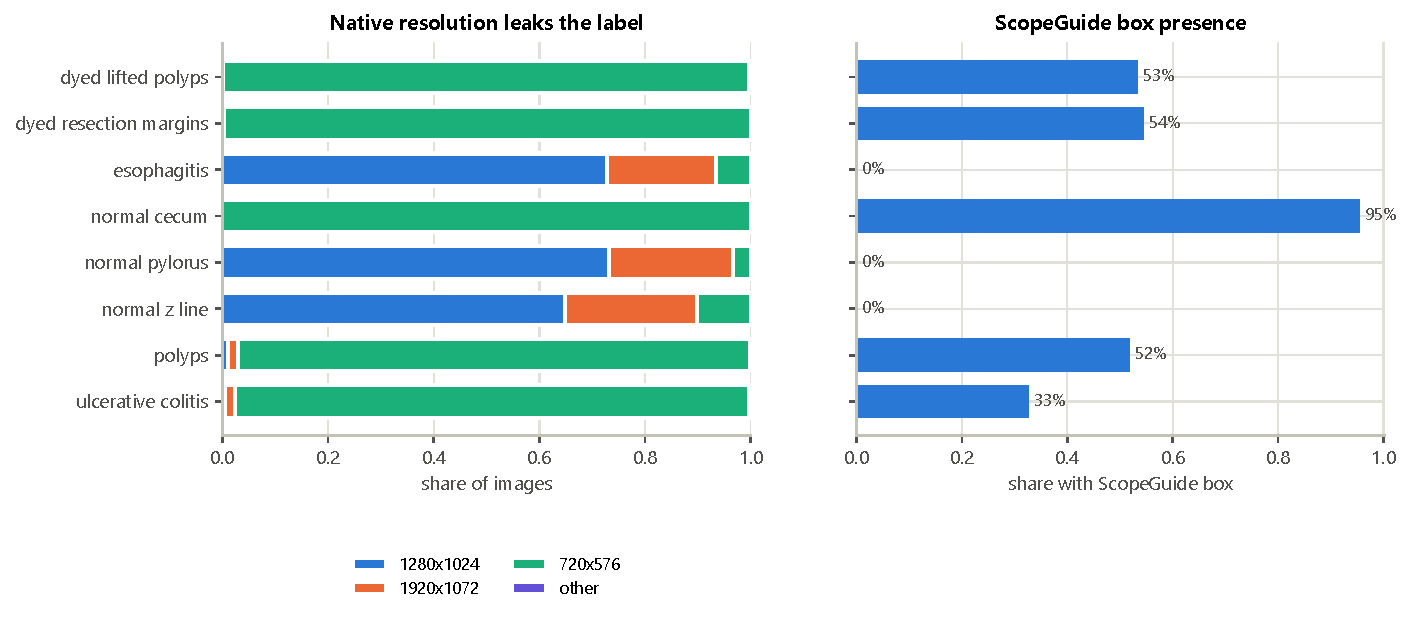
\includegraphics[width=0.95\linewidth]{eda_artefacts.pdf}
\caption{Acquisition artefacts by class: native-resolution mix (left) and presence of the ScopeGuide box (right).}
\end{figure}
\begin{figure}[h]
\centering
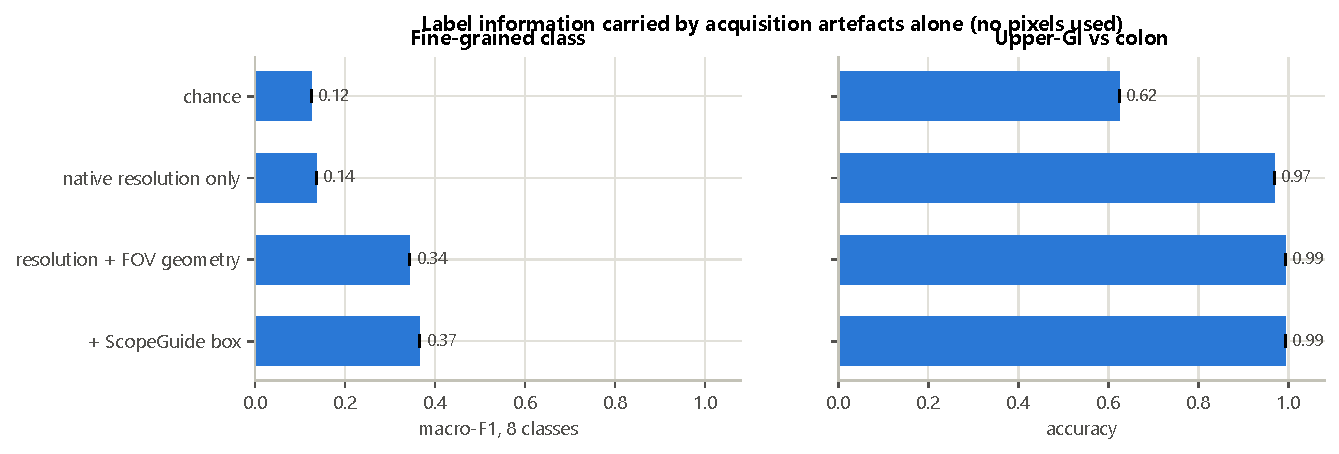
\includegraphics[width=0.8\linewidth]{eda_shortcut_probe.pdf}
\caption{Label information available from acquisition artefacts alone, using no pixel values. A gradient-boosted classifier on native resolution separates
upper-GI from colon frames with \resOnlyAcc{} accuracy, and with FOV geometry \resGeomAcc{}.}
\end{figure}

\section{Canonicalisation}
The endoscopic field of view is the largest bright blob after morphological opening (which strips thin text strokes); its convex hull gives the FOV
mask and the crop box. A rectangle covering the ScopeGuide location (measured on 419 detected boxes) is blacked out in every frame, and the \emph{valid}
mask excludes FOV exterior and this rectangle. Figure~\ref{fig:pipeline} shows the stages on three frames.

\begin{figure*}[t]
\centering
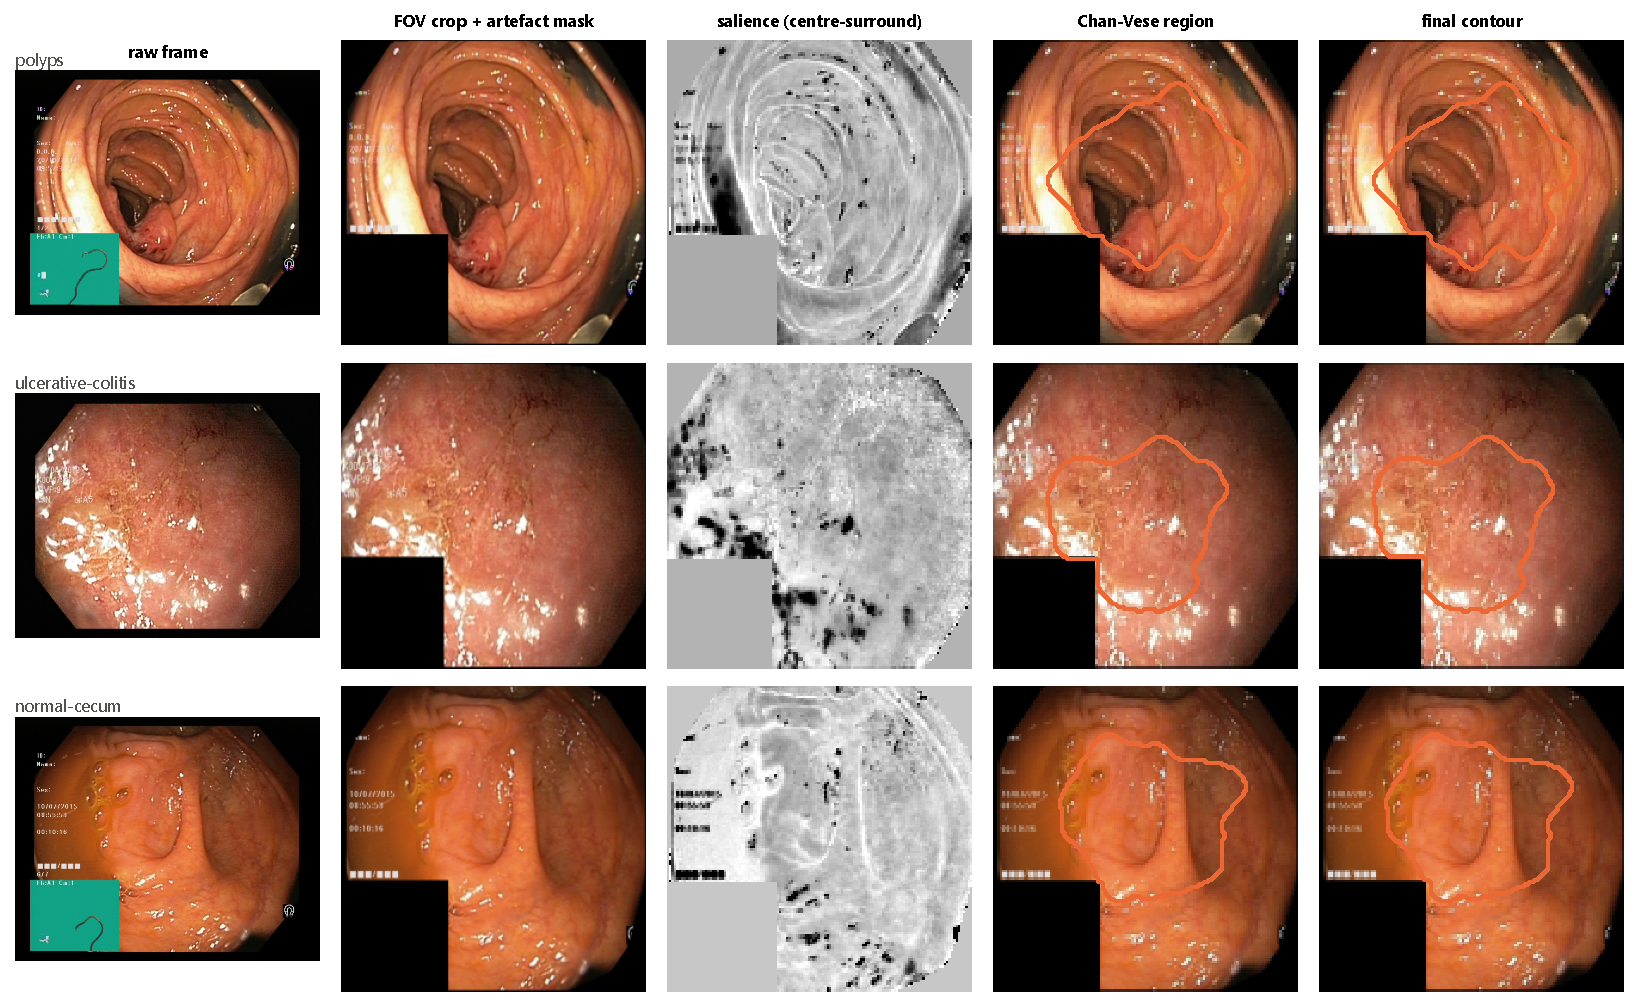
\includegraphics[width=0.9\linewidth]{ac_pipeline.pdf}
\caption{Pipeline illustration on a polyp, a colitis and a cecum frame: raw frame, FOV crop with artefact mask, centre--surround salience map, Chan--Vese region and final contour.}
\label{fig:pipeline}
\end{figure*}

\section{De-duplication, scene groups and splits}
Frozen DINOv2-S/14 embeddings give cosine similarity. Inspection of sampled pairs showed that similarity $\ge 0.95$ is the same frame, while 0.88--0.95
is the same lesion or lumen from a slightly different pose (consecutive frames of one procedure). Single-linkage at 0.90 chains into a 546-image blob, so the
group threshold is 0.92, giving \nGroups{} groups (largest 7). A stratified group split yields 5{,}578 / 797 / 1{,}594 train / val / test images with zero
group or hash overlap. A naive stratified random split with the same sizes would put \randLeakGroups{} groups on both sides of train/test; \randLeakPct{}
of its test images have a twin in the training set at similarity $\ge 0.92$. Near-duplicate leakage is therefore modest, and we report that size honestly.

\section{Distributions and collinearity}
Mean luma is close to normal (Shapiro--Wilk $p=0.16$), Laplacian variance is right-skewed (skew 1.36) and used on a log scale. The 98 contour-derived
features are heavily collinear (median VIF \vifMedian{}, \nVifTen{} features with VIF above 10), so regularised linear models and trees are used and
individual coefficients are never interpreted.

\begin{figure}[h]
\centering
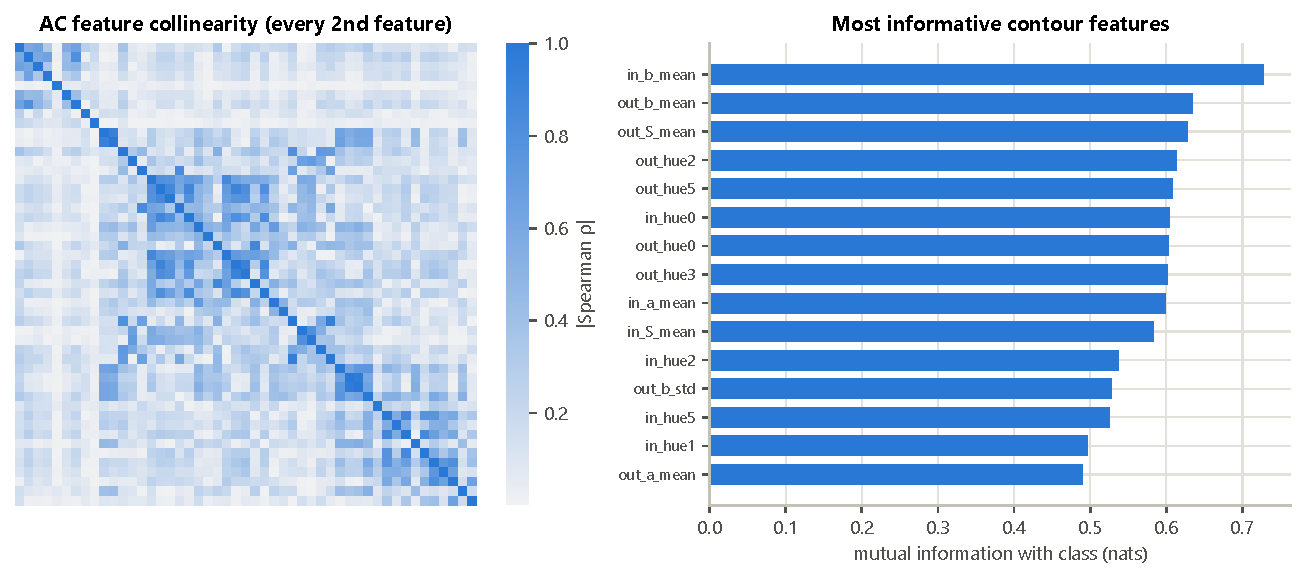
\includegraphics[width=0.95\linewidth]{eda_features.pdf}
\caption{Left: collinearity of the contour features. Right: mutual information of the most informative features with the class.}
\end{figure}
\begin{figure}[h]
\centering
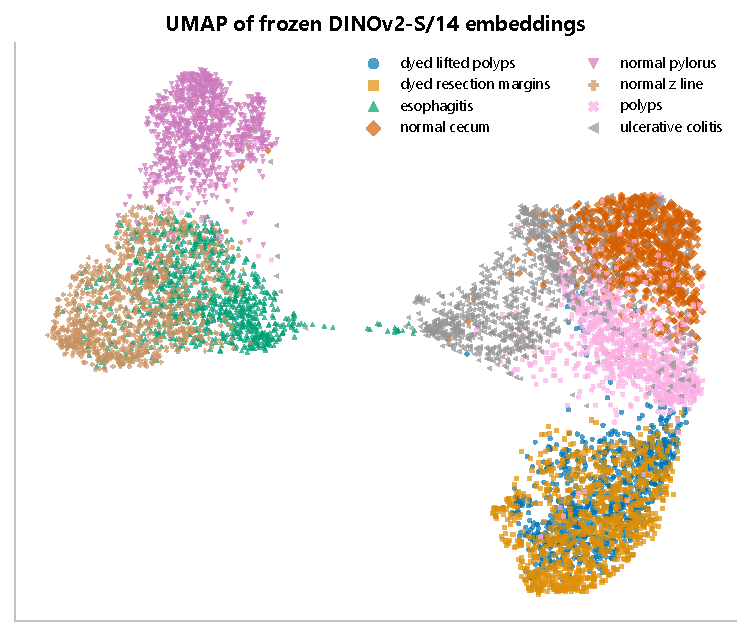
\includegraphics[width=0.6\linewidth]{eda_umap.pdf}
\caption{UMAP of frozen DINOv2 embeddings coloured by class (distinct marker shapes as a second channel).}
\end{figure}


\chapter{The Study: Related Work, Method, Experiments and Results}
\input{sections/related}
\input{sections/method}
\input{sections/setup}
\input{sections/results}
\input{sections/discussion}

\chapter{Engineering, Testing and Deployment}
\section{Repository architecture}
\begin{itemize}
\item \texttt{src/acpolyp/data}: download, ingestion, canonicalisation, curation, dataset and GPU augmentation.
\item \texttt{src/acpolyp/ac}: salience, two-stage morphological active contour, 136 features, tuning against Kvasir-SEG, extraction.
\item \texttt{src/acpolyp/models}: ACGNet and ablation modes, backbone factory, frozen-embedding extraction.
\item \texttt{src/acpolyp/training}: engine (AMP, warm-up/cosine, clipping, early stopping), metrics, calibration, conformal, classical baselines.
\item \texttt{src/acpolyp/evaluation}: paired statistics, aggregation across seeds, Grad-CAM, figure style.
\item \texttt{src/acpolyp/app}: FastAPI service and single-page frontend; \texttt{inference.py} shares the training preprocessing.
\item \texttt{scripts/}: experiment table, analysis, figure and paper-asset generation, model bundling, robustness, interpretability, the master script.
\item \texttt{tests/}: 48 automated tests.
\end{itemize}

\section{Engineering decisions driven by evidence}
\begin{description}
\item[GPU augmentation.] DataLoader workers are spawned (not forked) on Windows and each costs about 2.4\,GB of commit memory. With train, validation and test
loaders persistent, 18 workers exhausted the commit limit (Windows error 1455) and a run hung. Augmentation now runs on the GPU as one affine warp
shared by image, contour mask and valid mask, which is faster, removes worker processes and gives the web server the identical evaluation transform.
\item[Lazy memory-mapped caches.] Pickling a 1.5\,GB array into spawned workers failed; datasets now pickle as file paths and open memory maps on first access.
\item[Unit tests as a safety net.] They caught (i) a wrong DeLong AUC (midranks sliced in the wrong order), (ii) YAML 1.1 reading \texttt{1e-3} as a string,
(iii) a misleading gradient-flow check, because timm zero-initialises the last batch-norm gain of each residual block, so those branches legitimately have zero
gradient at step~0, and (iv) a duplicate-ID defect in the dataset itself via the data contract.
\item[Train/serve parity.] The bundle is re-run on raw test JPEGs through the complete preprocessing path and compared image by image with the logits saved at training
time: 100\,\% argmax agreement, mean absolute probability difference $2.5{\times}10^{-4}$ (bf16 versus fp32 arithmetic).
\end{description}

\section{Reproducibility}
Every run directory stores its configuration, git commit, command line, environment, per-epoch history, logits and summary. Seeds cover Python, NumPy,
PyTorch and CUDA; cuDNN is deterministic. \texttt{torch.use\_deterministic\_algorithms} is enabled with \texttt{warn\_only}, so a few CUDA kernels remain
non-deterministic: bit-exact replay is not guaranteed, which is why seed-to-seed spread is reported everywhere. \texttt{requirements.txt} freezes the
environment and \texttt{scripts/run\_experiments.ps1} rebuilds everything from an empty checkout.

\section{Web application}
A FastAPI backend (\texttt{/api/predict}, \texttt{/api/results}, \texttt{/api/health}, \texttt{/api/samples}) serves a dependency-free single-page frontend with a live demo
(calibrated probabilities, polyp probability against the validation-tuned threshold, conformal prediction set, contour and Grad-CAM overlays), a pipeline explainer,
a results dashboard rendered from the exported JSON, the data audit and an honesty section. Uploads are processed in memory and never stored. The page states
prominently that it is a research prototype.

\section{Packaging}
\texttt{scripts/build\_bundle.py} writes \texttt{outputs/artifacts/acpolyp-v1/}: weights (\texttt{safetensors}), configuration, scaler, calibration
(temperature, polyp threshold, conformal quantile), a model card and SHA-256 hashes. Selection of the bundled model uses \emph{validation} macro-F1 only.


\appendix
\chapter{Compliance with the 85-step workflow}
\begin{longtable}{p{0.05\linewidth}p{0.25\linewidth}p{0.14\linewidth}p{0.46\linewidth}}
\toprule \# & Step & Status & Where / note \\ \endhead
\midrule\multicolumn{4}{l}{\textbf{Phase I: Problem formulation, ML framing, feasibility}}\\\midrule
1 & Domain discovery; why rules fail & done & \texttt{docs/FORMULATION.md} \S{}1 (heuristic baseline measured) \\
2 & Task framing, \texttt{f\_\ensuremath{\theta}: X\ensuremath{\rightarrow}Y} & done & \S{}2 \\
3 & Objectives, RQs, H0/H1 & done & \S{}3 (RQ1--RQ5) \\
4 & Metric taxonomy (+ cost matrix) & done & \S{}4; \texttt{scripts/analyze.py} (5:1 cost operating point) \\
5 & Data/compute/latency feasibility & done & \S{}5 \\
6 & Scope, non-goals, MVM vs stretch & done & \S{}6 \\
\midrule\multicolumn{4}{l}{\textbf{Phase II: Literature, SOTA, baselines}}\\\midrule
7 & Literature survey & done & \texttt{docs/LITERATURE.md}, \texttt{paper/references.bib} (verified entries) \\
8 & Codebase / model-zoo audit & done, limitation & \S{}3 of LITERATURE; no official Kvasir baselines exist to re-run (optional item n/a) \\
9 & Benchmark \& leaderboard audit & done, limitation & \S{}1, \S{}4 of LITERATURE; no verifiable public leaderboard for this protocol \\
10 & Gap synthesis \& contributions & done & \S{}5 of LITERATURE; paper \S{}I \\
\midrule\multicolumn{4}{l}{\textbf{Phase III: Governance, licensing, planning}}\\\midrule
11 & Work breakdown \& roadmap & done & this file, \texttt{scripts/run\_deep.py} (declarative experiment table), \texttt{scripts/run\_experiments.ps1} \\
12 & Risk register \& fallback & done & \texttt{docs/FORMULATION.md} \S{}7 \\
13 & PII sanitisation & n/a (conditional (public images, no user text)) & EXIF/comment scan: 0/8000 hits (\texttt{data/ingest.py}); burned-in text discussed in \texttt{docs/DATA\_AUDIT.md} \\
14 & Licence audit & done & \texttt{docs/LICENSING.md} \\
\midrule\multicolumn{4}{l}{\textbf{Phase IV: Environment}}\\\midrule
15 & Repo structure, git, ignores & done & standard layout; \texttt{.gitignore}; \texttt{ruff} configured in \texttt{pyproject.toml}; \texttt{.pre-commit-config.yaml} \\
16 & Locked environment & done & \texttt{.venv}, \texttt{requirements.txt} (frozen), \texttt{pyproject.toml} \\
17 & GPU/OS configuration & done & CUDA torch 2.11+cu128 verified; Windows-specific fixes documented (spawn, commit limit) \\
18 & Run logging & done & \texttt{runlog.py}: config, git hash, command, environment, CSV/JSON per run. TensorBoard/MLflow optional n/a \\
\midrule\multicolumn{4}{l}{\textbf{Phase V: Acquisition}}\\\midrule
19 & Verified idempotent download & done & \texttt{data/download.py} (byte count, SHA-256, zip test, zip-slip guard, resume) \\
20 & Ingestion into canonical schema & done & \texttt{data/ingest.py} (images \ensuremath{\rightarrow} uint8 caches + parquet; no CSV/JSONL inputs exist) \\
\midrule\multicolumn{4}{l}{\textbf{Phase VI: Ground truth}}\\\midrule
21 & Labelling schema & n/a (conditional (dataset labels used as given)) & class taxonomy in \texttt{data/contracts.py}; boundary cases (esophagitis\ensuremath{\leftrightarrow}z-line) in the audit \\
22 & Self-annotated gold set & n/a (optional (no clinical expertise to annotate honestly)) & Kvasir-SEG expert masks serve as the gold set for the contour stage \\
23 & Programmatic labelling & n/a (optional) & cleanlab used for *flagging*, not relabelling \\
\midrule\multicolumn{4}{l}{\textbf{Phase VII: Cleaning and QA}}\\\midrule
24 & Sanitisation & done & decode check, valid-FOV, artefact masking (\texttt{data/preprocess.py}) \\
25 & Duplicates & done & SHA-256 + embedding cosine (pHash evaluated and rejected, with evidence) \\
26 & Outliers / label noise & done & range checks, IQR blur outliers, \texttt{cleanlab} (550 flagged) \\
27 & Schema validation & done & \texttt{data/contracts.py} (pydantic + assertions); it caught the duplicate-ID defect \\
\midrule\multicolumn{4}{l}{\textbf{Phase VIII: EDA}}\\\midrule
28 & Distributions, normality & done & \texttt{scripts/eda.py}; \texttt{docs/DATA\_AUDIT.md} \S{}4 \\
29 & Imbalance, subgroups & done & 1.007 (8-class), 1:7 (polyp-vs-rest), per-format and per-box subgroups \\
30 & Collinearity, shortcuts & done & VIF, Spearman, MI; resolution/box probes \\
31 & Manifold & done & UMAP (\texttt{outputs/figures/eda\_umap.*}) \\
\midrule\multicolumn{4}{l}{\textbf{Phase IX: Splits and leakage}}\\\midrule
32 & Deterministic split & done & stratified group split, seed 42; random split as control; OOD hold-out optional n/a \\
33 & Leakage audit & done & \texttt{curate.leakage\_audit}; zero group/hash overlap asserted \\
34 & CV folds & done & 5 grouped folds serialised (\texttt{cv\_fold}), used for out-of-fold label-noise estimation \\
35 & Versioned artefacts & done & \texttt{data/processed/{train,val,test}\_ids.txt} + SHA-256 in \texttt{curation\_report.json}; Arrow/HDF5 optional n/a (memory-mapped \texttt{.npy} used) \\
\midrule\multicolumn{4}{l}{\textbf{Phase X: Features and preprocessing}}\\\midrule
36 & Scaling & done & train-only 1/99 winsorise + z-score (\texttt{dataset.fit\_scaler}); power transforms optional n/a \\
37 & Categorical/temporal encoding & n/a & no such features \\
38 & Domain features, selection & done, limitation & 136 features (colour, LBP, GLCM, shape, boundary); importance by MI and SHAP rather than pruning \\
39 & Tokenisation & n/a & vision task \\
40 & Augmentation & done & GPU affine + colour jitter, contour mask follows geometry (\texttt{data/augment.py}, tested) \\
41 & Imbalance mitigation & n/a & classes balanced; polyp-vs-rest handled by threshold tuning, not resampling \\
42 & Pipeline serialisation & done & \texttt{scaler.json}, \texttt{calibration.json}, \texttt{config.yaml} inside each bundle \\
\midrule\multicolumn{4}{l}{\textbf{Phase XI: Modelling}}\\\midrule
43--46 & Formulation, loss, architecture, parameters/VRAM & done & \texttt{docs/FORMULATION.md} \S{}8; \texttt{models/acgnet.py}; measured params and VRAM in profiling table \\
\midrule\multicolumn{4}{l}{\textbf{Phase XII: Skeleton and baselines}}\\\midrule
47 & Dataset/DataLoader & done & \texttt{data/dataset.py} (uint8 contract, in-process loader; spawn workers rejected on Windows) \\
48 & Walking skeleton & done & \texttt{tests/test\_walking\_skeleton.py} (constant model, real loader, runs in seconds) \\
49 & Trivial \& heuristic baselines & done & random, prior, Lab-centroid heuristic (\texttt{classical.run\_trivial}) \\
50 & Classical baselines & done & LR, RBF-SVM, RF, LightGBM, XGBoost \\
51 & Pretrained / confidence baselines & done & frozen-DINOv2 linear probe; max-softmax risk--coverage \\
\midrule\multicolumn{4}{l}{\textbf{Phase XIII: Implementation}}\\\midrule
52 & Config schema & done & \texttt{configs/*.yaml} + dotted CLI overrides (unit-tested; caught the YAML \texttt{1e-3} string bug) \\
53 & Modular architecture, hooks & done & \texttt{ACGNet}; forward hooks for Grad-CAM and layer-wise probes \\
54 & Metrics & done & \texttt{training/metrics.py} (\texttt{ignore\_index} n/a no padding) \\
55 & Optimiser, scheduler, clipping & done & AdamW, no decay on bias/norm, warm-up + cosine, clip 1.0 \\
56 & Train/eval loops & done & \texttt{training/engine.py} (accumulation optional n/a not needed) \\
57 & Seeding & done, limitation & all RNGs seeded; cuDNN deterministic; \texttt{use\_deterministic\_algorithms(warn\_only=True)}, so a few CUDA kernels remain non-deterministic (bit-exact replay is not guaranteed; seed-to-seed spread is reported) \\
58 & Checkpoint, early stopping & done & best \texttt{.safetensors} by val macro-F1, patience 4 \\
\midrule\multicolumn{4}{l}{\textbf{Phase XIV: Debugging}}\\\midrule
59 & Shape/device asserts & done & in \texttt{ACGNet.forward}, \texttt{predict} (finite logits) and tests \\
60 & Single-batch overfit & done & \texttt{tests/test\_model\_sanity.py} \\
61 & Gradient flow & done & test (after one step, because timm zero-inits last BN gains); grad norm logged each epoch \\
62 & Numerical stability & done & fp32 loss on bf16 logits, finite asserts, stable softmax \\
63 & Unit tests & done & 48 tests; batch-order invariance included \\
\midrule\multicolumn{4}{l}{\textbf{Phase XV: Optimisation}}\\\midrule
64 & AMP, SDPA, cached features & done & bf16 autocast; timm fused attention for ViT/Swin; cached frozen embeddings \\
65 & PEFT & limitation (optional) & frozen-backbone linear probe only; LoRA not used \\
66 & HPO & done, limitation & Optuna/TPE on validation for the contour (80 trials) and classical models (25 each); deep nets use one shared recipe. A learning-rate sweep (seed 0) and a post hoc 3-seed replication at 2x LR quantify what that costs: the plain model improves by 0.8 points at 2x LR and the guided-vs-plain gap stays null \\
67 & Ensembling & done & seed and backbone soft-voting \\
\midrule\multicolumn{4}{l}{\textbf{Phase XVI: Post-processing}}\\\midrule
68 & Threshold tuning & done & Youden J on validation (+ cost-optimal threshold) \\
69 & Calibration & done & temperature scaling, reliability diagrams, ECE, Brier \\
70 & Uncertainty & done & split-conformal (LAC), risk--coverage \\
\midrule\multicolumn{4}{l}{\textbf{Phase XVII: Evaluation}}\\\midrule
71 & Locked test evaluation & done & test touched once per frozen run; secondary dataset optional n/a (HyperKvasir overlaps) \\
72 & Multi-seed & done & deep N=3, classical N=5, mean \ensuremath{\pm} SD \\
73 & Significance & done & paired bootstrap (2,000), McNemar, DeLong, Holm, Cohen's d, seed-level tests \\
74 & Ablations & done & 7 variants + 3 controls \\
75 & Sensitivity, scaling, Pareto & done & learning curves, LR sweep, accuracy--latency \\
76 & OOD / perturbation & done & JPEG compression and Gaussian blur on 480 stratified frames, 3 seeds x 5 variants incl. controls (\texttt{scripts/robustness2.py}); single-seed noise/blur/brightness/JPEG screen (\texttt{scripts/robustness.py}, helper) \\
77 & Profiling & done & latency (warm-up + sync), VRAM, train time, checkpoint size \\
\midrule\multicolumn{4}{l}{\textbf{Phase XVIII: Interpretability and errors}}\\\midrule
78 & Confusion, per-class, ROC/PR & done & \texttt{analyze.py} \\
79 & Failure taxonomy & done & error gallery + automated categories (label-flagged, confusable pairs) + manual inspection notes in the report \\
80 & Attribution & done & TreeSHAP, Grad-CAM (pointing game vs expert masks) \\
81 & Layer-wise probes & done & per-stage linear probes, pretrained vs fine-tuned \\
82 & Subgroup audit & done & by scope format, ScopeGuide box, class; worst-group accuracy \\
\midrule\multicolumn{4}{l}{\textbf{Phase XIX: Packaging}}\\\midrule
83 & One-command CLI & done & \texttt{scripts/run\_experiments.ps1}; entry points \texttt{scripts/train.py}, \texttt{scripts/evaluate.py}, \texttt{scripts/predict.py} (wrappers over \texttt{acpolyp.training.train} / \texttt{acpolyp.cli}), \texttt{python -m acpolyp.cli serve} \\
84 & Bundle + local UI & done & \texttt{outputs/artifacts/acpolyp-v1/} (weights, scaler, calibration, model card, hashes); FastAPI + custom single-page UI (instead of Gradio) \\
\midrule\multicolumn{4}{l}{\textbf{Phase XX: Documentation and archival}}\\\midrule
85 & README, figures/tables script, manuscript, slides, clean-room check & done, limitation & \texttt{README.md}; \texttt{scripts/make\_figures.py} (runs EDA, contour, analysis, export, paper-asset scripts: 300-dpi vector PDFs, \texttt{booktabs} tables with bold-best and \ensuremath{\pm} SD); \texttt{paper/main.tex} (IEEEtran, 7 pp.); \texttt{report/report.pdf} (34 pp.); \texttt{slides/ACPolyp.pptx} (13 slides); clean-room clone + install + 48 tests run locally (the 8 h pipeline was not re-run from scratch). Publishing to GitHub/Zenodo/Hugging Face is left to the owner (needs their accounts) \\
\bottomrule\end{longtable}


\chapter{Failure Taxonomy of the Most Confident Errors}
The 36 most confident errors of the seed-ensembled ACG-ConvNeXt (117 errors in total on the test split) were inspected and sorted into four categories.
\emph{The categories are visual judgements by the project author, who is not a clinician; they are not a clinical adjudication and should be reviewed by a gastroenterologist.}
\begin{table}[h]
\centering\small
\begin{tabular}{p{0.2\linewidth}rrp{0.5\linewidth}}
\toprule
Category & $n$ & flagged & What the frames show \\
\midrule
A. Esophagitis $\leftrightarrow$ z-line & 17 & 15 & Irregular, inflamed or whitish mucosa at or near the gastro-oesophageal junction; both labels plausible, esophagitis is defined relative to the z-line. \\
B. Dyed lifted $\leftrightarrow$ resection margin & 7 & 5 & Blue-dye craters or lifted lesions at different stages of endoscopic resection; the visible state often supports either label. \\
C. ``Polyp'' predicted as another class & 7 & 2 & Frames labelled polyps with no distinct visible lesion (homogeneous mucosa) or a small or marginal lesion; predicted cecum, colitis or pylorus. The clinically important group. \\
D. Other & 5 & 4 & Diffuse redness labelled colitis predicted as cecum or esophagitis; a snare loop with bleeding. \\
\bottomrule
\end{tabular}
\caption{Failure taxonomy of the 36 most confident errors; ``flagged'' = flagged by confident learning. Overall 26 of 36 are flagged, against about 5\,\% of correct predictions.}
\end{table}

\chapter{Additional Figures}
\begin{figure}[h]
\centering
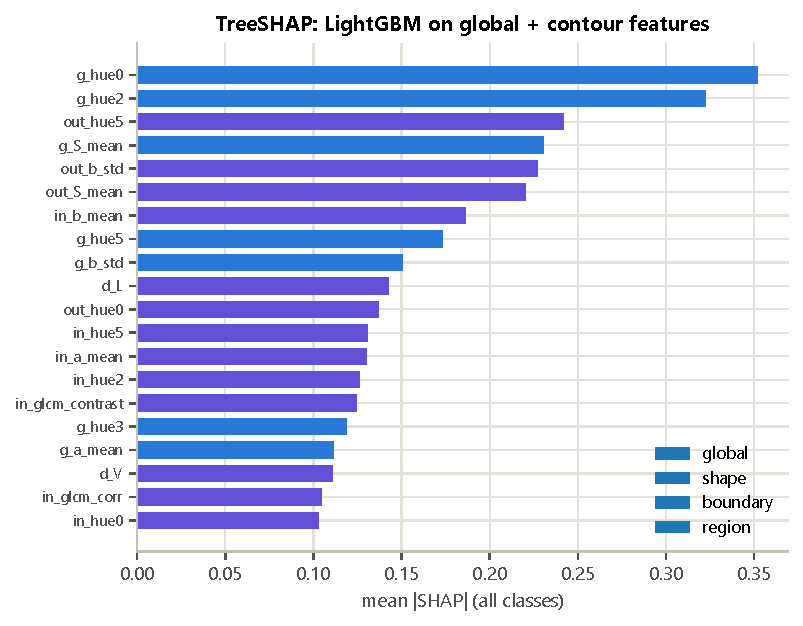
\includegraphics[width=0.7\linewidth]{shap_top20.pdf}
\caption{TreeSHAP importance of the 20 most influential features of the LightGBM model on global and contour features (all classes). Region (inside/outside colour and texture) and global colour features dominate; contour shape and boundary features contribute about \shapShape{} and \shapBoundary{} of the total.}
\end{figure}
\begin{figure}[h]
\centering
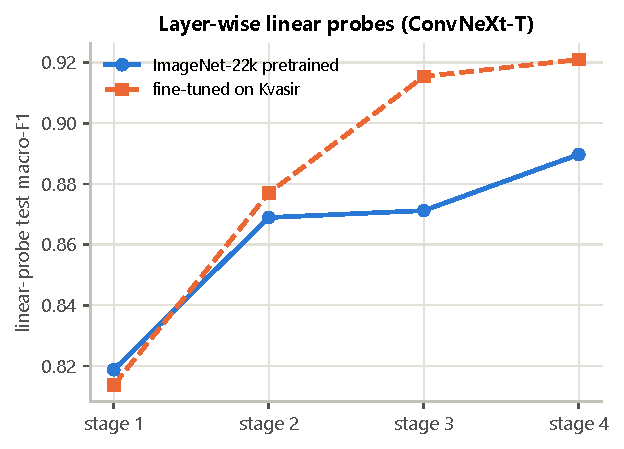
\includegraphics[width=0.55\linewidth]{layerwise_probe.pdf}
\caption{Layer-wise linear probes on ConvNeXt-T stages: ImageNet-22k pretrained versus fine-tuned on Kvasir. Fine-tuning mostly reshapes the last two stages.}
\end{figure}
\begin{figure}[h]
\centering
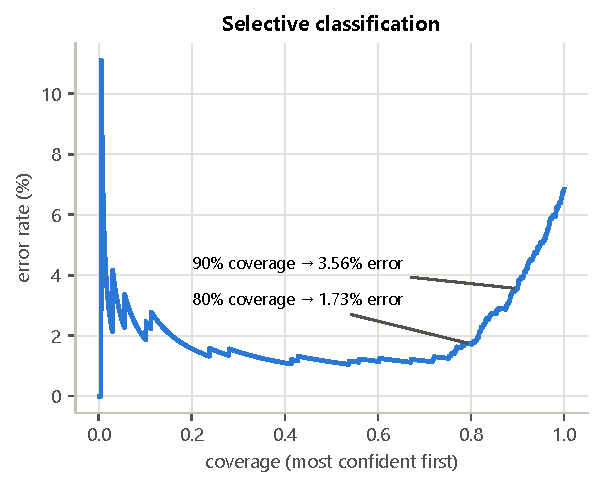
\includegraphics[width=0.5\linewidth]{risk_coverage.pdf}
\caption{Selective classification: error rate on the most confident fraction of test frames (ACG-ConvNeXt, seed 0).}
\end{figure}
\begin{figure}[h]
\centering
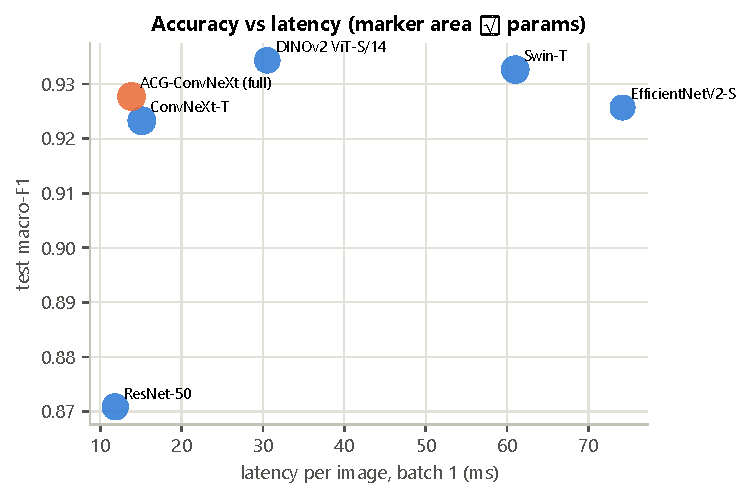
\includegraphics[width=0.55\linewidth]{pareto.pdf}
\caption{Accuracy--latency trade-off (batch-1 latency on an RTX~4060 Laptop GPU; marker area proportional to parameter count).}
\end{figure}
\begin{figure}[h]
\centering
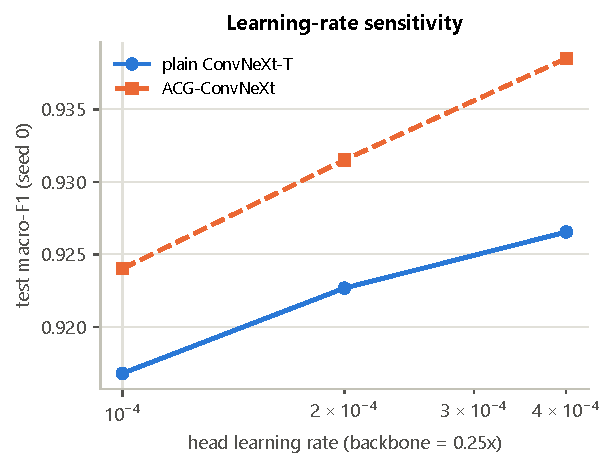
\includegraphics[width=0.5\linewidth]{lr_sensitivity.pdf}
\caption{Learning-rate sensitivity for plain and guided ConvNeXt-T (seed 0). A three-seed replication at twice the default rate is reported in Section~\ref{sec:data} of the results text.}
\end{figure}
\begin{figure}[h]
\centering
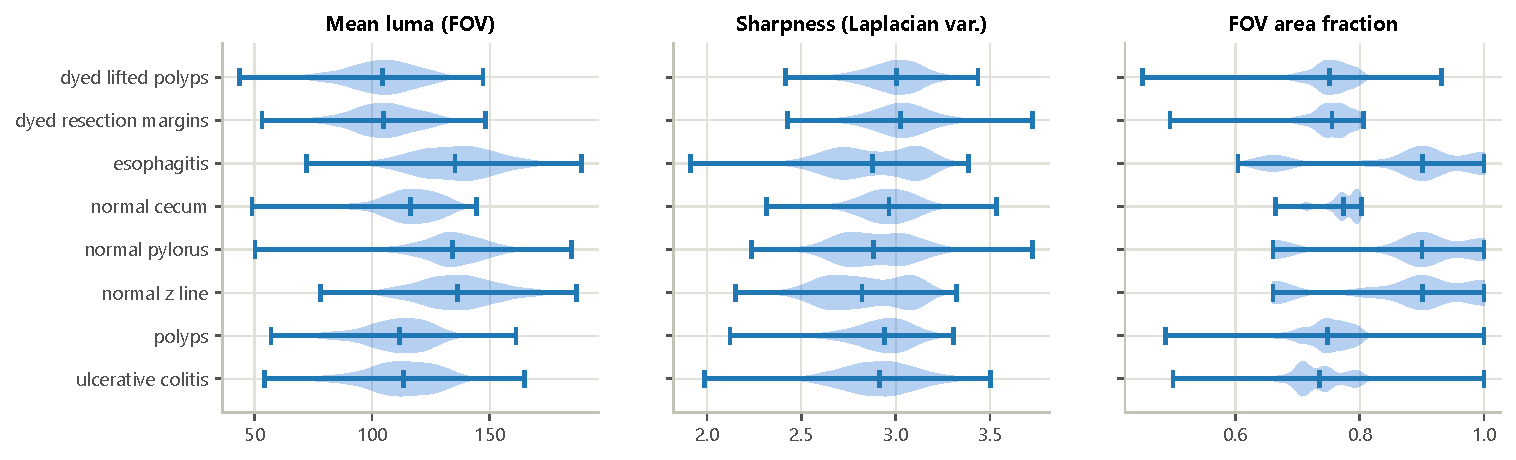
\includegraphics[width=0.9\linewidth]{eda_image_stats.pdf}
\caption{Image statistics by class: mean luma, sharpness and field-of-view fraction.}
\end{figure}
\begin{figure}[h]
\centering
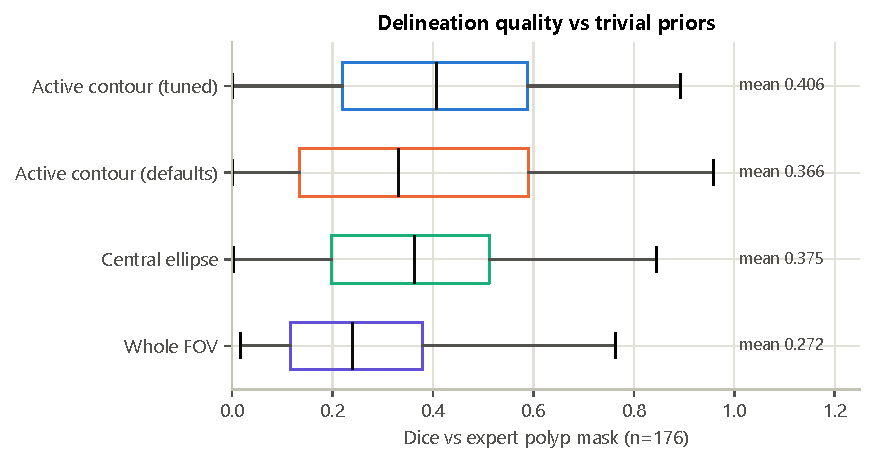
\includegraphics[width=0.6\linewidth]{ac_dice_boxplot.pdf}
\caption{Delineation quality: tuned contour versus trivial priors on 176 expert-masked test-split polyps.}
\end{figure}


\bibliographystyle{plain}
\bibliography{references}
\end{document}
